\documentclass[journal,11pt]{IEEEtran}
% --------------------
\usepackage{ifpdf}
\usepackage{cite}
\ifCLASSINFOpdf
   \usepackage[pdftex]{graphicx}
\usepackage{amsmath}
\usepackage{algorithmic}
\usepackage{array}
\usepackage{url}
% --------------------
\usepackage{booktabs} 
\usepackage{float}
\usepackage{hyperref}
\usepackage{multirow}
\usepackage{amssymb}
\usepackage{subcaption}
% --------------------
\begin{document}
\title{Online Debate in Times of Crisis:\\ \normalsize{\textit{Examining the evolution of debate fragmentation in the Iranian Twitter sphere during the Coronavirus quarantine}}}
% --------------------
\author{Farzam Fanitabasi
\thanks{Social Data Science Course Project, \today}}
% --------------------
\maketitle
% --------------------
\IEEEpeerreviewmaketitle
% --------------------
\section{Introduction}
\label{S:Intro}
\IEEEPARstart{M}{odern} societies are becoming increasingly polarised, where identity politics and ideologies fragment the society into subgroups~\cite{gillani2018me}. 
In the context of online social media discussions (such as micro-blogging websites like twitter), the general pattern across these fragmented subgroups indicates that the majority of communication happens internally (within the group) rather than between different groups~\cite{garcia2015ideological}. Often, these groups are fragmented among religious beliefs, political party lines, and ideological views~\cite{bright2018explaining}. However, epidemic breakouts do not distinguish people based on their beliefs and group belongings. Often, such situations enforce a heightened emotional and mental distress on the society. In the past, wars and epidemics have managed to blur the fragmentation lines, and bring communities and nations together in solidarity~\cite{}. \\

This project studies the evolution of debate fragmentation during the Coronavirus quarantine in Iran, aiming to determine whether a significant change in debate structure and groups occur as the quarantine period progresses. The motivation behind this is to analyse whether more challenging and stressful times can act as a binding factor between people (by blurring party lines), or the fragmentation and polarisation remain unchanged, if not stronger. The scope of this project concerns the Iranian Twitter-sphere. To study the group fragmentation within this sphere, three different hashtags are used, addressing different debate topics with various levels of political controversy. These three topics are examined in two weeks, to analyse the possible changes in fragmentation.
% --------------------
\subsection{Data Retrieval \& Processing}
\label{S:DR}
% --------------------
This project studies three different topics, discussed between March $26^{th}$ till April $13^{th}$ on the Iranian Twitter sphere.
The selected topics, represented as hashtags $\#$ in Twitter, possess an inherent controversy with them, ranging from low, to medium, to high controversy.
The reason behind choosing three topics with varying controversy level is to analyse whether the fragmentation and its possible evolution depends on the underlying controversy of the topic.
The first topic, focuses on the general discussion around the Coronavirus, and is represented by \#Corona (in Persian). The reactions to this topic varies mildly across the supporters and opposition to the Iranian government, as the measures, policies, and lack of quarantine have been subject to discussions in the society. The second topic, focuses on the tweets about the Iranian president, who became the chief coordinator for the Corona measures. The tweets are collected using \#Rouhani (in Persian). During the first few weeks of the outbreak in Iran, he was under scrutiny and criticism from both sides for his reaction to the situation. The last topic, and the one with the most controversy, is the presence of doctors without borders (Médecins Sans Frontières) in Iran, collected using \#MSD (in Persian). The controversy\footnote{\href{https://www.doctorswithoutborders.org/what-we-do/news-stories/story/iranian-authorities-revoke-approval-msf-coronavirus-treatment-center}{https://www.doctorswithoutborders.org/what-we-do/news-stories/story/iranian-authorities-revoke-approval-msf-coronavirus-treatment-center}}, resulted in their short stay in Iran, and quick expulsion from the country. The reasons behind this expulsion and the rationality of this act was highly debated at the time in Iran. The tweet datasets for each topic is gathered via the Rtweet package in R. To further analyse the debate and its fragmentation given different modes of interaction, out of each dataset two different networks/graphs are created: (i) \emph{Endorsement Network}, and (ii) \emph{Reply Network}. For each network, the unique users involved in the debate are extracted, and for each user their (maximum) 2000 most recent tweets are collected, forming their interaction timeline. For the first network, the timelines are filtered to only contain users who have retweeted each other in the past. In literature, such retweet network is known as the \emph{Endorsement Network}~\cite{morgan2013news,colleoni2014echo}'. For the second network, the timelines are filtered to only contain users that have replied to each other, known as the \emph{Reply Network}. Table~\ref{T:datasets} presents detailed information about the collected datasets.
%%%%
%%%%
%%%%
\begin{table*}[!htb]
\centering
\caption{Collected datasets, generated networks, their sizes, and order}
\scriptsize
\begin{tabular}{lllllll}
\toprule
\textbf{Dataset / Measure} & \textbf{Corona 26.03} & \textbf{Corona 13.04} & \textbf{Rouhani 26.03} & \textbf{Rouhani 13.04} &\textbf{MSF 26.03} & \textbf{MSF 13.04} \\
\midrule
\textbf{Hashtag (in Persian)} & \#Corona & \#Corona & \#Rouhani & \#Rouhani & \#MSD & \#MSD  \\
\addlinespace
\textbf{Political Controversy} & Medium & Medium & Low & Low & High & High \\
\addlinespace
\textbf{Original $\#$ of Tweets} & 5,636,281 & 4,597,322 & 1,329,335 & 1,327,388 & 2,324,405 & 103,976\\
\addlinespace
\textbf{Original $\#$ of Users} & 5,200  & 4,245 & 1,260 & 1,269 & 1,577 & 101 \\
\addlinespace
\textbf{$\#$ of Vertices (Endorsement Network)} & 5,200  & 4,245 & 1,260 & 1,269 & 1,577 & 101\\
\addlinespace
\textbf{$\#$ of Edges (Endorsement Network)} &  201,680 & 164,431 & 18,146 & 16,359 & 63,489 & 688\\
\addlinespace
\textbf{$\#$ of Vertices (Reply Network)} & 5,200  & 4,245 & 1260 & 1,269 & 1,577 & 101 \\
\addlinespace
\textbf{$\#$ of Edges (Reply Network)} & 252,296  & 165,641 & 27,800 & 19,101 & 86,055 & 154\\
\bottomrule
\end{tabular}
\label{T:datasets}
\end{table*}
%%%%
%%%%
%%%%
% --------------------
\section{Methodology}
\label{S:Method}
% --------------------
To analyse and evaluate the evolution of fragmentation, the resulting 12 networks (3 topics, 2 snapshots, endorsement/reply) are studied given various visualisations, descriptive, structural metrics. In the first step, using the Rtweet package and the Gephi software, the 12 networks are visualised. To improve the presentation and quality, all network are visualised using the \textit{Fruchterman Reingold} layout, and coloured by their modularity class\footnote{Additionally, nodes are resized based on their betweenness centrality.}. Figure~\ref{fig:graphsEN} and Figure~\ref{fig:graphsRN} illustrate the endorsement and reply networks, respectively. Where the top row shows the networks generated on 2020.3.26, and the lower row are the networks generated on 2020.4.13. \\

In the second step, a subset of descriptive and structural metrics and measures are selected to analyse and study each network. These metrics include network diameter, average path, edge density, compactness, modularity, and assortativity coefficient. In the case of the latter, it is calculated using the ``$assortativity_{nominal}$" function, with node communities as the attribute. The results of applying these metrics are presented in Table~\ref{T:measuresEN} for the endorsement network, and Table~\ref{T:measuresRN} for the reply network. \\

In the last step, to compare the endorsement and reply network, for each metrics $M$, the relative difference between the two networks are calculated as $(M_{en} - M_{rn}) / M_{en}$, where $M_{en}$ is the calculated metric for the endorsement network, and $M_{rn}$ represents the same calculated metric for the reply network.
% --------------------
\section{Analysis \& Evaluation}
\label{S:Anal}
% --------------------
\subsection{Permutation Testing}
\label{S:PT}
% --------------------
The first step in analysing the networks, is to compare them to a random network with the same degree distribution (null hypothesis testing). As the most important metric in the analysis is the modularity of the networks, these experiments compare the generated network modularity with a random network. The p-value of these experiments are illustrated in Table~\ref{T:pVal}. The results indicate that the generated networks are significantly more modular than the random networks.
%%%%
%%%%
%%%%
\begin{table}[t]
\centering
\caption{Permutation Testing: 1000 iterations each network given random edge sampling. The Perm. modularity is the average of the 1000 iterations.}
\scriptsize
\resizebox{\linewidth}{!}{%
\begin{tabular}{lllll}
\toprule
\textbf{Interaction} & \textbf{Network} & \textbf{Modularity} & \textbf{Perm. Modularity} & \textbf{P-Value} \\
\midrule
\textbf{Endorsement} & \textbf{Corona 03.26} & 0.6321 & 0.0646 & 0*** \\
\addlinespace
& \textbf{Corona  04.13} & 0.675 & 0.0642 & 0*** \\
\addlinespace
& \textbf{Rouhani 03.26} & 0.6626 & 0.1081 & 0*** \\
\addlinespace
& \textbf{Rouhani  04.13} & 0.6619 & 0.1089 & 0*** \\
\addlinespace
& \textbf{MSF 03.26} & 0.601 &  &  \\
\addlinespace
& \textbf{MSF 04.13} & 0.6196 &  &  \\
\addlinespace
\midrule
\addlinespace
\textbf{Reply} & \textbf{Corona 03.26} & 0.484 & 0.0629 & 0*** \\
\addlinespace
& \textbf{Corona 04.13} & 0.5021 & 0.0693 & 0*** \\
\addlinespace
& \textbf{Rouhani 03.26} & 0.5103 & 0.092 & 0*** \\
\addlinespace
& \textbf{Rouhani 04.13} & 0.5763 & 0.106 & 0 \\
\addlinespace
& \textbf{MSF 03.26} & 0.4632 &  &  \\
\addlinespace
& \textbf{MSF 04.13} & 0.5593 &  &  \\
\addlinespace
\bottomrule
\end{tabular}}
\label{T:pVal}
\end{table}
%%%%
%%%%
%%%%
\begin{figure*}[!htb]
\centering
\subfloat[\#Corona 2020.03.26]{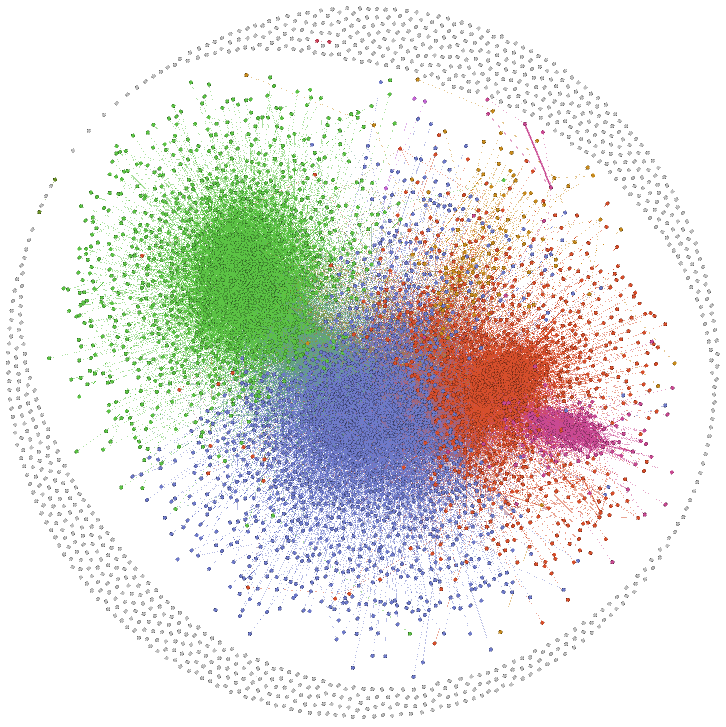
\includegraphics[width =0.25\textwidth]{figures/Corona2603.png}}\hspace{0.01\textwidth}
\subfloat[\#Rouhani 2020.03.26]{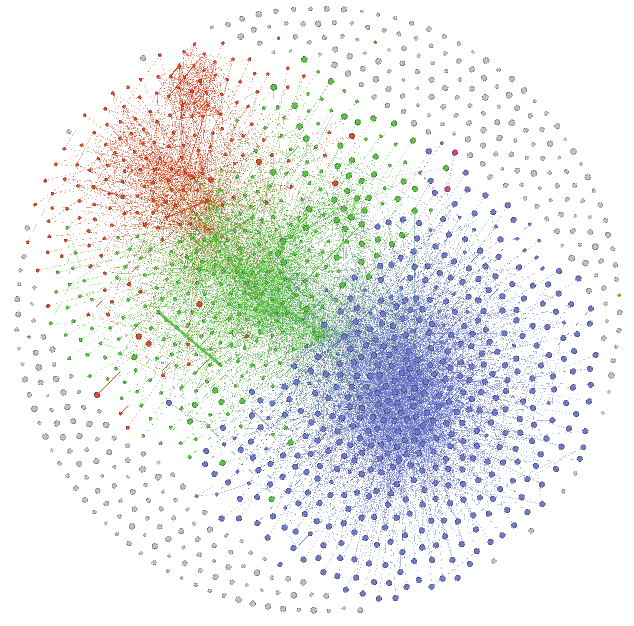
\includegraphics[width = 0.25\textwidth]{figures/rouhani2603.png}}\hspace{0.01\textwidth}
\subfloat[\#MSF 2020.03.26]{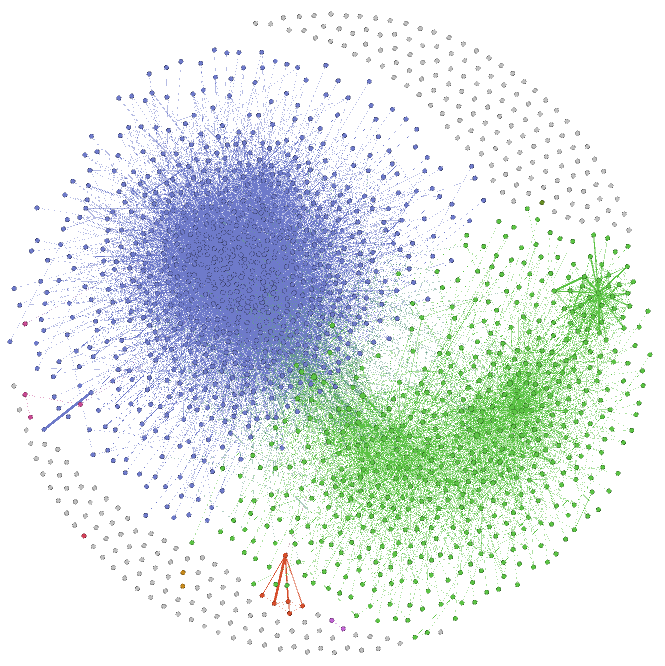
\includegraphics[width =0.25\textwidth]{figures/Sans2603.png}} \\[2ex]
\subfloat[\#Corona 2020.04.13]{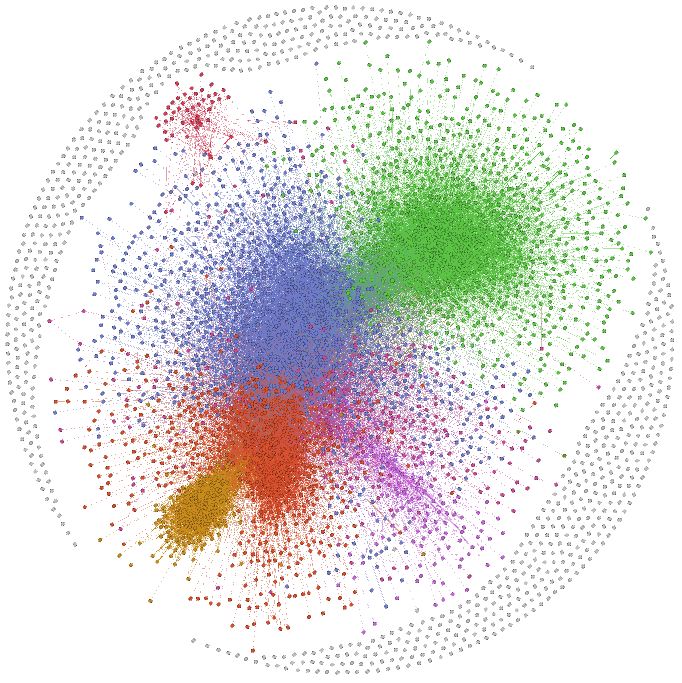
\includegraphics[width = 0.25\textwidth]{figures/Corona1304.png}}\hspace{0.01\textwidth}
\subfloat[\#Rouhani 2020.04.13]{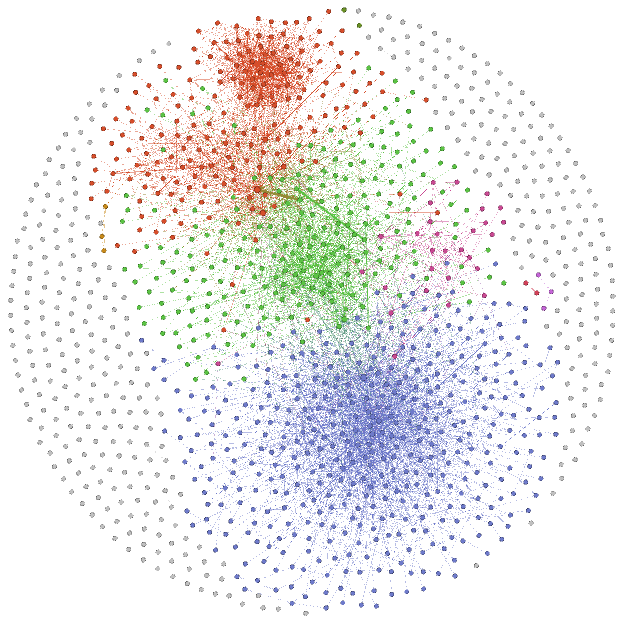
\includegraphics[width =0.25\textwidth]{figures/rouhani1304.png}}\hspace{0.01\textwidth}
\subfloat[\#MSF 2020.04.13]{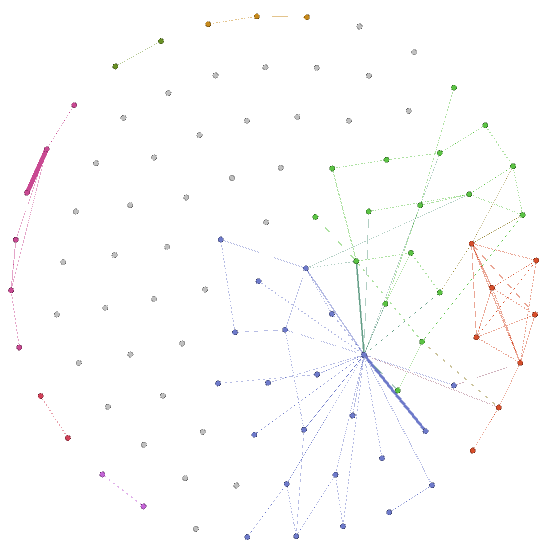
\includegraphics[width = 0.25\textwidth]{figures/Sans1304.png}}
\caption{Endorsement Network}
\label{fig:graphsEN}
\end{figure*}
%%%%
%%%%
%%%%
\begin{table*}[t]
\centering
\caption{Topological Metrics for Different Datasets: \textbf{Endorsement Network}}
\scriptsize
\resizebox{\linewidth}{!}{%
\begin{tabular}{llllllll}
\toprule
\textbf{Dataset / Metric} &  & \textbf{Corona 26.03} & \textbf{Corona 13.04} & \textbf{Rouhani 26.03} & \textbf{Rouhani 13.04} &\textbf{MSF 26.03} & \textbf{MSF 13.04} \\
\midrule
\textbf{General Descriptive} & \textbf{Diameter} & 8 & 8 & 7 & 8 & 8 & 5 \\
\addlinespace
 & \textbf{Average Path} & 3.042 & 3.167 & 3.1632 & 3.4207 & 3.0243 & 2.7841 \\
\midrule
\textbf{Interconnectedness} & \textbf{Edge Density} & 0.014 & 0.018 & 0.0228 & 0.0203 & 0.0511 & 0.1362 \\
\addlinespace
 & \textbf{Mean Degree} & 77.5 & 77.47 & 28.8 & 25.78 & 80.56 & 13.62 \\
\addlinespace
 & \textbf{Compactness} & 0.2397028 & 0.2249 & 0.1959 &  0.153 & 0.2587 & 0.0953 \\
\midrule
\textbf{Centralisation} & \textbf{Betweenness: mean | sd} & 3605.4 | 16645.3 & 3039.9 | 13035.6 & 772.3 |  2974.4 & 731.1 | 2872.7 & 1126.7 | 3689.4 & 20.2 | 88.9 \\
%\addlinespace
% & \textbf{Closeness Centrality (sd)} & 6.573358e-08* & 9.368537e-0* & 8.204772e-07* & 6.34478e-07* & 7.685997e-07* & 4.14284e-05* \\
\addlinespace
 & \textbf{Compactness} & 0.2397028 & 0.2249 & 0.1959 &  0.153 & 0.2587 & 0.0953 \\
\addlinespace
 & \textbf{Eigenvector centrality: sd} & 0.0257741 & 0.0222 & 0.0398 & 0.0495 & 0.0391 & 0.1399 \\
 \midrule
 \textbf{Structural Metrics} & \textbf{Connected Components} & 910 & 791 & 312 & 387 & 250 & 44 \\
 \addlinespace
 & \textbf{Avg. Clustering Coefficient} & 0.196 & 0.2053 & 0.209 & 0.2073 & 0.2342 & 0.266 \\
\addlinespace
 & \textbf{Modularity} & 0.6321 & 0.675 & 0.6626 & 0.6619 & 0.601 & 0.6196 \\
 \addlinespace
 & \textbf{Assortativity Coefficient} & 0.8188 & 0.8383 & 0.8181 & 0.8829 & 0.7732 & 0.9425 \\
 \addlinespace
\bottomrule
\end{tabular}}
\label{T:measuresEN}
\end{table*}
%%%%
%%%%
%%%%
% --------------------
\subsection{Fragmentation over Time}
\label{S:FoT}
% --------------------
\begin{figure*}[t]
\centering
\subfloat[\#Corona 2020.03.26]{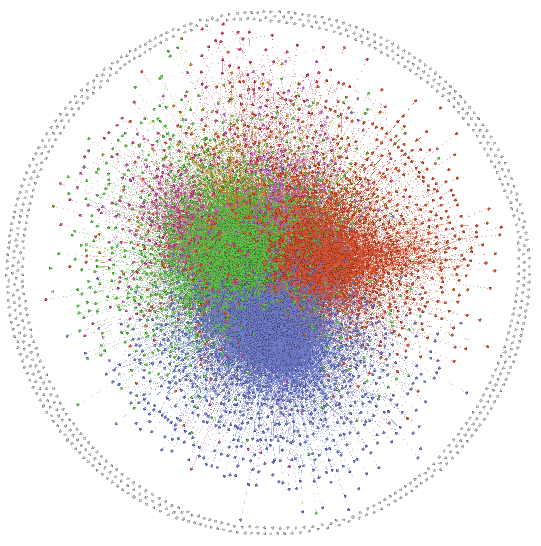
\includegraphics[width =0.25\textwidth]{figures/Corona2603Reply.png}}\hspace{0.01\textwidth}
\subfloat[\#Rouhani 2020.03.26]{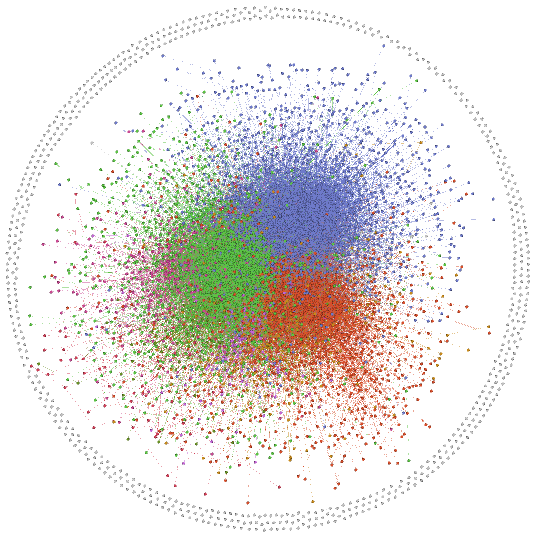
\includegraphics[width = 0.25\textwidth]{figures/Rouhani2603Reply.png}}\hspace{0.01\textwidth}
\subfloat[\#MSF 2020.03.26]{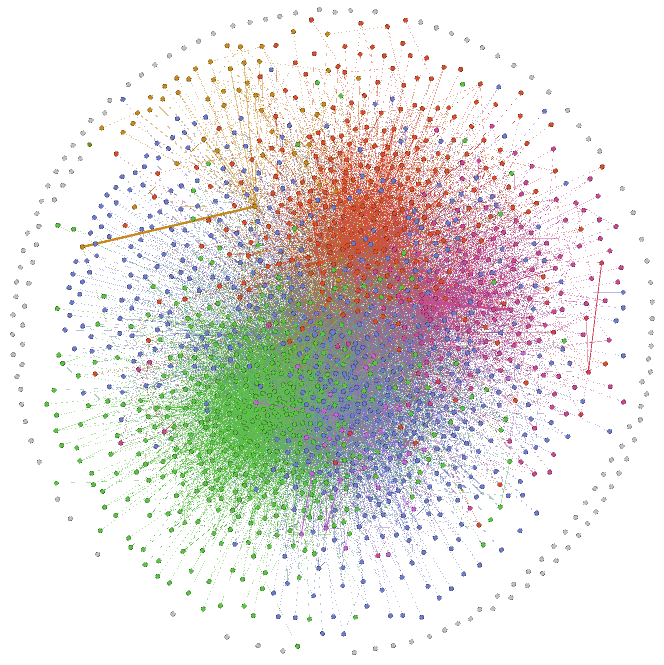
\includegraphics[width =0.25\textwidth]{figures/Sans2603Reply.png}} \\[2ex]
\subfloat[\#Corona 2020.04.13]{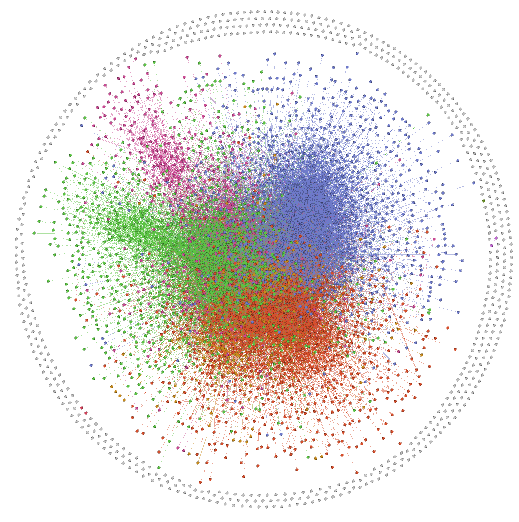
\includegraphics[width = 0.25\textwidth]{figures/Corona1304Reply.png}}\hspace{0.01\textwidth}
\subfloat[\#Rouhani 2020.04.13]{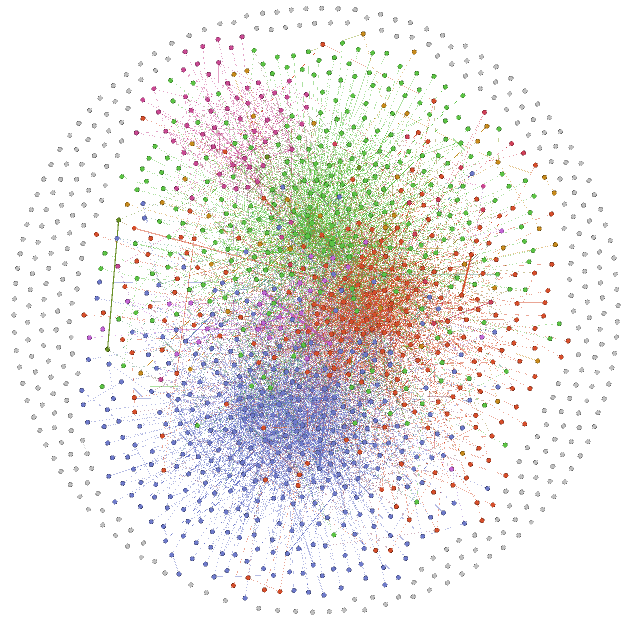
\includegraphics[width =0.25\textwidth]{figures/Rouhani1304Reply.png}}\hspace{0.01\textwidth}
\subfloat[\#MSF 2020.04.13]{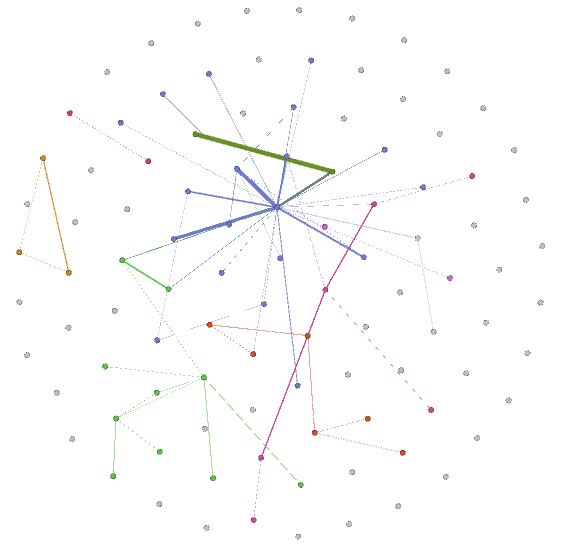
\includegraphics[width = 0.25\textwidth]{figures/Sans1304Reply.png}}
\caption{Reply Network}
\label{fig:graphsRN}
\end{figure*}
%%%%
%%%%
%%%%
\begin{table*}[t]
\centering
\caption{Topological Metrics for Different Datasets: \textbf{Reply Network}}
\scriptsize
\resizebox{\linewidth}{!}{%
\begin{tabular}{llllllll}
\toprule
\textbf{Dataset / Metric} &  & \textbf{Corona 26.03} & \textbf{Corona 13.04} & \textbf{Rouhani 26.03} & \textbf{Rouhani 13.04} &\textbf{MSF 26.03} & \textbf{MSF 13.04} \\
\midrule
\textbf{General Descriptive} & \textbf{Diameter} & 7 & 8 & 7 & 8 & 6 & 9 \\
\addlinespace
 & \textbf{Average Path} & 2.775 & 2.898 & 2.8286 & 3.0746 & 2.4971 & 3.6737 \\
\midrule
\textbf{Interconnectedness} & \textbf{Edge Density} & 0.0186 & 0.01838 & 0.035 & 0.0237 & 0.0693 & 0.0304 \\
\addlinespace
 & \textbf{Mean Degree} & 97.036 & 78.04 & 44.12 & 30.10402 & 109.2069 & 3.049 \\
\addlinespace
 & \textbf{Compactness} & 0.2397028 & 0.2249 & 0.1959 &  0.153 & 0.2587 & 0.0953 \\
\midrule
\textbf{Centralisation} & \textbf{Betweenness: max  |  sd} & 3555.9 | 25015.2 & 2914.3 | 15899.1 & 800.7 | 3394.8 & 743.1 | 3390.5 & 1000.7 | 10049.5 & 28.7 | 106.5 \\
%\addlinespace
% & \textbf{Closeness Centrality (sd)} & 8.667637e-08* & 1.121543e-07* & 1.162737e-06* & 8.04668e-07* & 1.244637e-06* & 3.945429e-05* \\
\addlinespace
 & \textbf{Compactness} & 0.297 & 0.2675 & 0.2655 & 0.1995 & 0.3635 & 0.0742 \\
\addlinespace
 & \textbf{Eigenvector centrality: sd} & 0.0232 & 0.0388 & 0.0573 & 0.04019 & 0.0489 & 0.14376 \\
 \midrule
 \textbf{Structural Metrics} & \textbf{Connected Components} & 632 & 633 & 209 & 315 & 125 & 52\\
 \addlinespace
 & \textbf{Avg. Clustering Coefficient} & 0.1489761 & 0.1369 & 0.1598 & 0.1527 & 0.2244 & 0.2967 \\
\addlinespace
 & \textbf{Modularity} & 0.484 & 0.5021 & 0.5103 & 0.5763 & 0.4632 & 0.5593 \\
 \addlinespace
 & \textbf{Assortativity Coefficient} & 0.6088 & 0.6128 & 0.6227 & 0.6574 & 0.5383 & 0.7892 \\
 \addlinespace
\bottomrule
\end{tabular}}
\label{T:measuresRN}
\end{table*}
%%%%
%%%%
%%%%
The evolution of debate fragmentation and polarisation across time have been subject to previous research~\cite{garimella2017long,yardi2010dynamic,barbera2014social,garcia2015ideological}. Such research have indicated that group polarisation changes, particularly among politicians, as they get closer to elections~\cite{lietz2014politicians}. Additionally, previous research such as~\cite{bright2018explaining} and~\cite{garcia2015ideological} have analysed the mass polarisation of public across time in different (mostly European) countries. However, no previous research has been done on Iranian twitter sphere, particularly in crisis and quarantine times. \\

Figures~\ref{fig:graphsEN} and~\ref{fig:graphsRN}, as well as Tables~\ref{T:measuresEN} and~\ref{T:measuresRN} present the visualised networks and the calculated metrics, respectively. Note that the generated networks are not limited to the debate topic, rather, each network illustrates the composition of the users involved in the debate, and their historical activity and interaction. Hence, the two snapshots indicate how (and if) the composition and interaction of the involved users in the debate evolves. \\

In all cases, the debates are very modular, and based on the assortativity index, highly fragmented. In the case of the Corona debate (Figure~\ref{fig:graphsEN}.a/d and~\ref{fig:graphsRN}.a/d), the passage of time created 1 more big community, and slight increase in modularity, without any significant changes in the overall structure of debate. The debate around the presidents (Figure~\ref{fig:graphsEN}.b/e and~\ref{fig:graphsRN}.b/e), the passage on time did not cause a significant change in modularity and assortativity. Lastly, in the case of the debate around Doctors without Borders (Figure~\ref{fig:graphsEN}.c/f and~\ref{fig:graphsRN}.c/f), initially the debate was highly fragmented across the two endorsement communities with very little endorsements (retweets) across the two main communities. However, in both the endorsement and reply networks, the debate very quickly died down and within 2 weeks, not many users are still discussing the issue.
%%%%
%%%%
%%%%
\begin{figure*}[t]
\centering
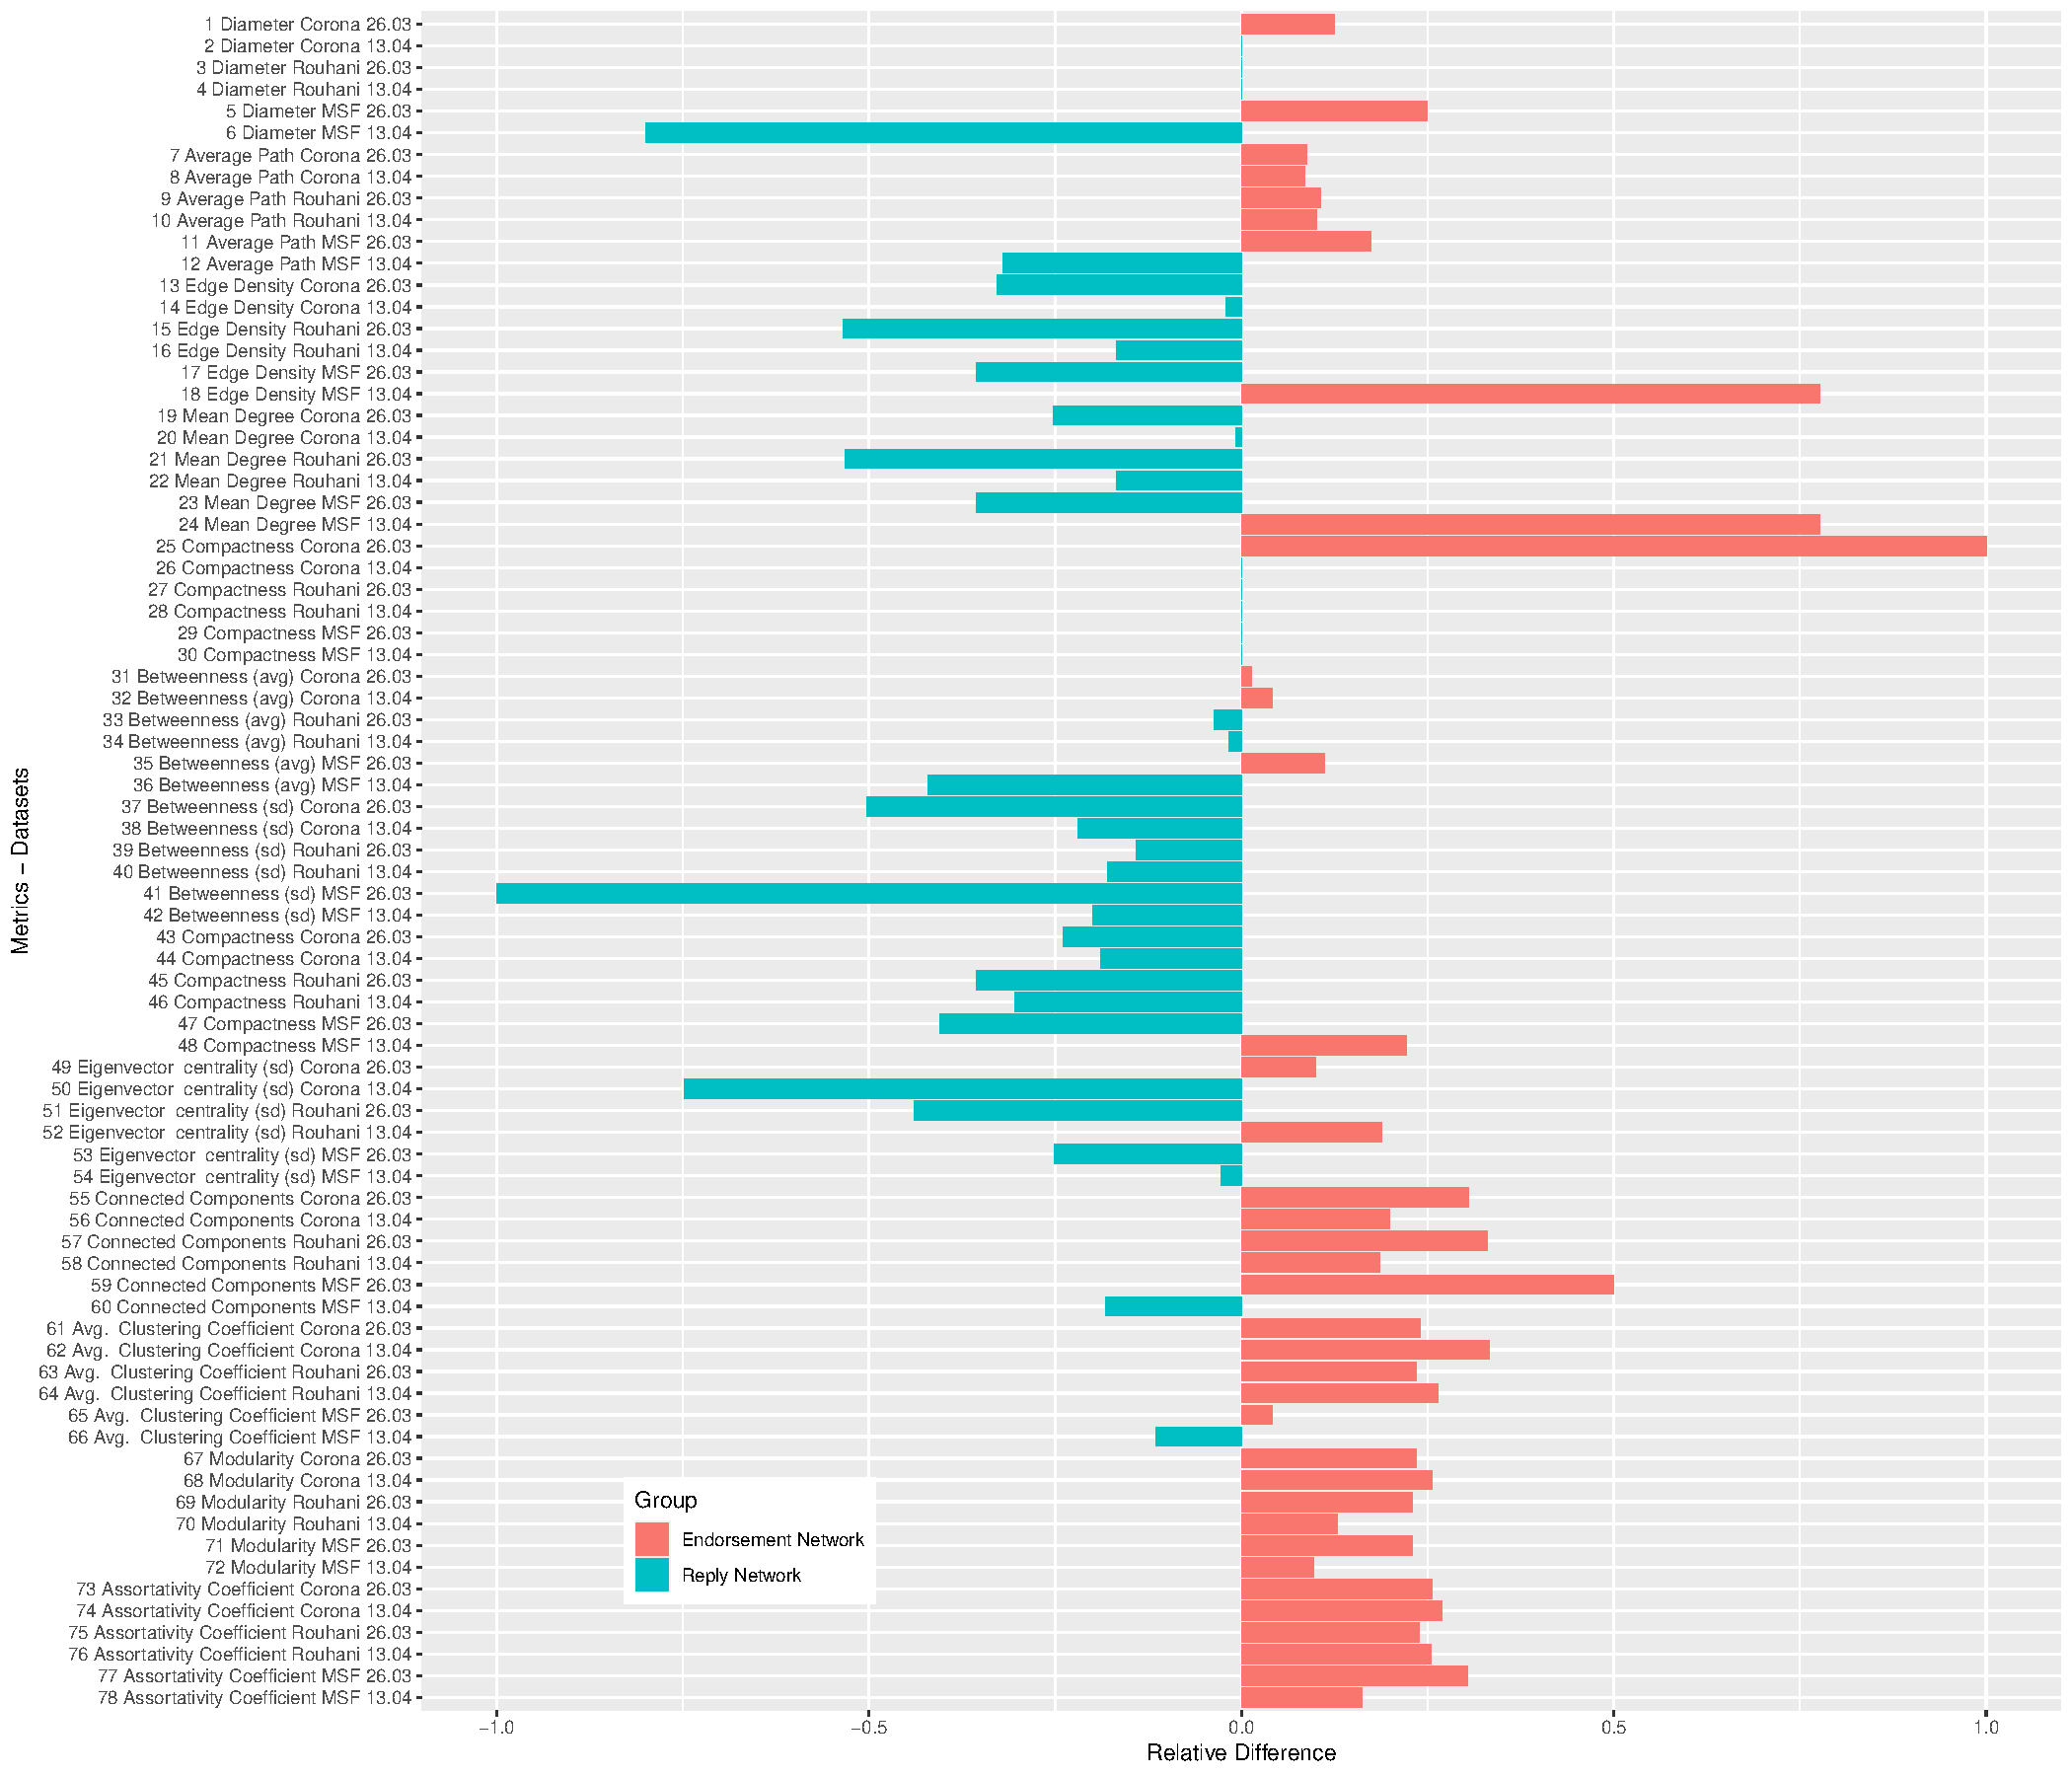
\includegraphics[width =1\linewidth]{figures/twoSidedBarPlot.pdf}
\caption{Reply Network}
\label{fig:barplot}
\end{figure*}
%%%%
%%%%
%%%%
% --------------------
\subsection{Comparing the Endorsement \& Reply Networks}
\label{S:CER}
% --------------------
Differences between the endorsement and reply networks in twitter have also been subject to previous research. Generally, the endorsement network which is based on retweets, shows more agreeable actions, while in reply networks, users tend to discuss and disagree with each other~\cite{himelboim2013tweeting,colleoni2014echo}. Rooted in social science, this difference is mainly due to the theory of selective exposure~\cite{himelboim2013tweeting}, and the law of group polarisation~\cite{sunstein1999law}. \\

The same difference, previously seen in US and German twitter spheres~\cite{gillani2018me,barbera2014social} can be seen in Iranian twitter sphere across all analysed debates. Where in comparison to the endorsement network, the debates are still modular, but have a lower assortativity score. This means that users from different communities engage (reply) with each other in higher volumes compared to the endorsement networks. Figures~\ref{T:measuresEN} and~\ref{fig:graphsRN} visualise the interactions among users in the reply networks. Again, it can be seen that compared to the endorsement networks, the users are interacting more with each other across different communities. \\

Lastly, to compare the endorsement and reply networks, Figure~\ref{fig:barplot} illustrates the relative differences between the two network across all 78 feature (13 metrics, 6 networks). As illustrated, the endorsement network is more modular and assortative, while the reply network is more interconnected. 
% --------------------
\subsection{Note on Centralisation \& Twitter Access in Iran}
Twitter is filtered in Iran by the government, and access to it is only possible using virtual private networks (VPNs) or by Iranians living abroad. However, the use of such anti-censorship tools is wide-spread. Additionally, while the access is restricted for the population, almost all Iranian official have twitter accounts, and actively use it to share news and their opinions. However, due to the special case of such censorship, many users avoid retweeting or replying to officials in Iran, hence the network is less dominated by individual users. This observation can be validated via the centralisation and interconnectedness metrics in Tables~\ref{T:measuresEN} and~\ref{T:measuresEN}.
% --------------------
\section{Limitations \& Critic}
\label{S:Conc}
This project was limited by few factors: (i) Lack of data collection facilities for twitter data without premium subscription. While collecting the datasets took around 2 days each time, the data is only a sample of the users involved in the debate. Additionally, the actual graph for the used hashtags given the same users is not available for normal twitter developers. Lastly, due to the filtering of twitter in Iran, location data is not a good condition for selecting data, nor are the hashtags themselves, as the words are often the same in Arabic and Persian Hence, few steps of preprocessing and filtering was needed to get correct tweets. (ii) Lack of sentiment analysis tools for Persian language. This fact hindered the community detection and analysis of the changing sentiments. Hence, this project was inspired by non-language specific approaches in the literature~\cite{chkhartishvili2018binary,garimella2017reducing}. \\

One critic to this project can be the lack of data, specifically the debate network in longer time periods. However, this can be remedied by using paid developer accounts in Tweeter. Additionally, while no significant changes in debate fragmentation and user composition were found during the two snapshots, given more complete data, the same methodology can provided more insight into the unexplored Iranian twitter sphere.
% --------------------
\medskip
\bibliographystyle{IEEEtran}
\bibliography{reference.bib}
% --------------------
\end{document}

\end{document}


